\section{Referencia de la Clase Cobros\-List}
\label{classCobrosList}\index{CobrosList@{CobrosList}}
Administra los datos de la lista de cobros.  


{\tt \#include $<$cobroslist.h$>$}

Diagrama de colaboraci\'{o}n para Cobros\-List:\begin{figure}[H]
\begin{center}
\leavevmode
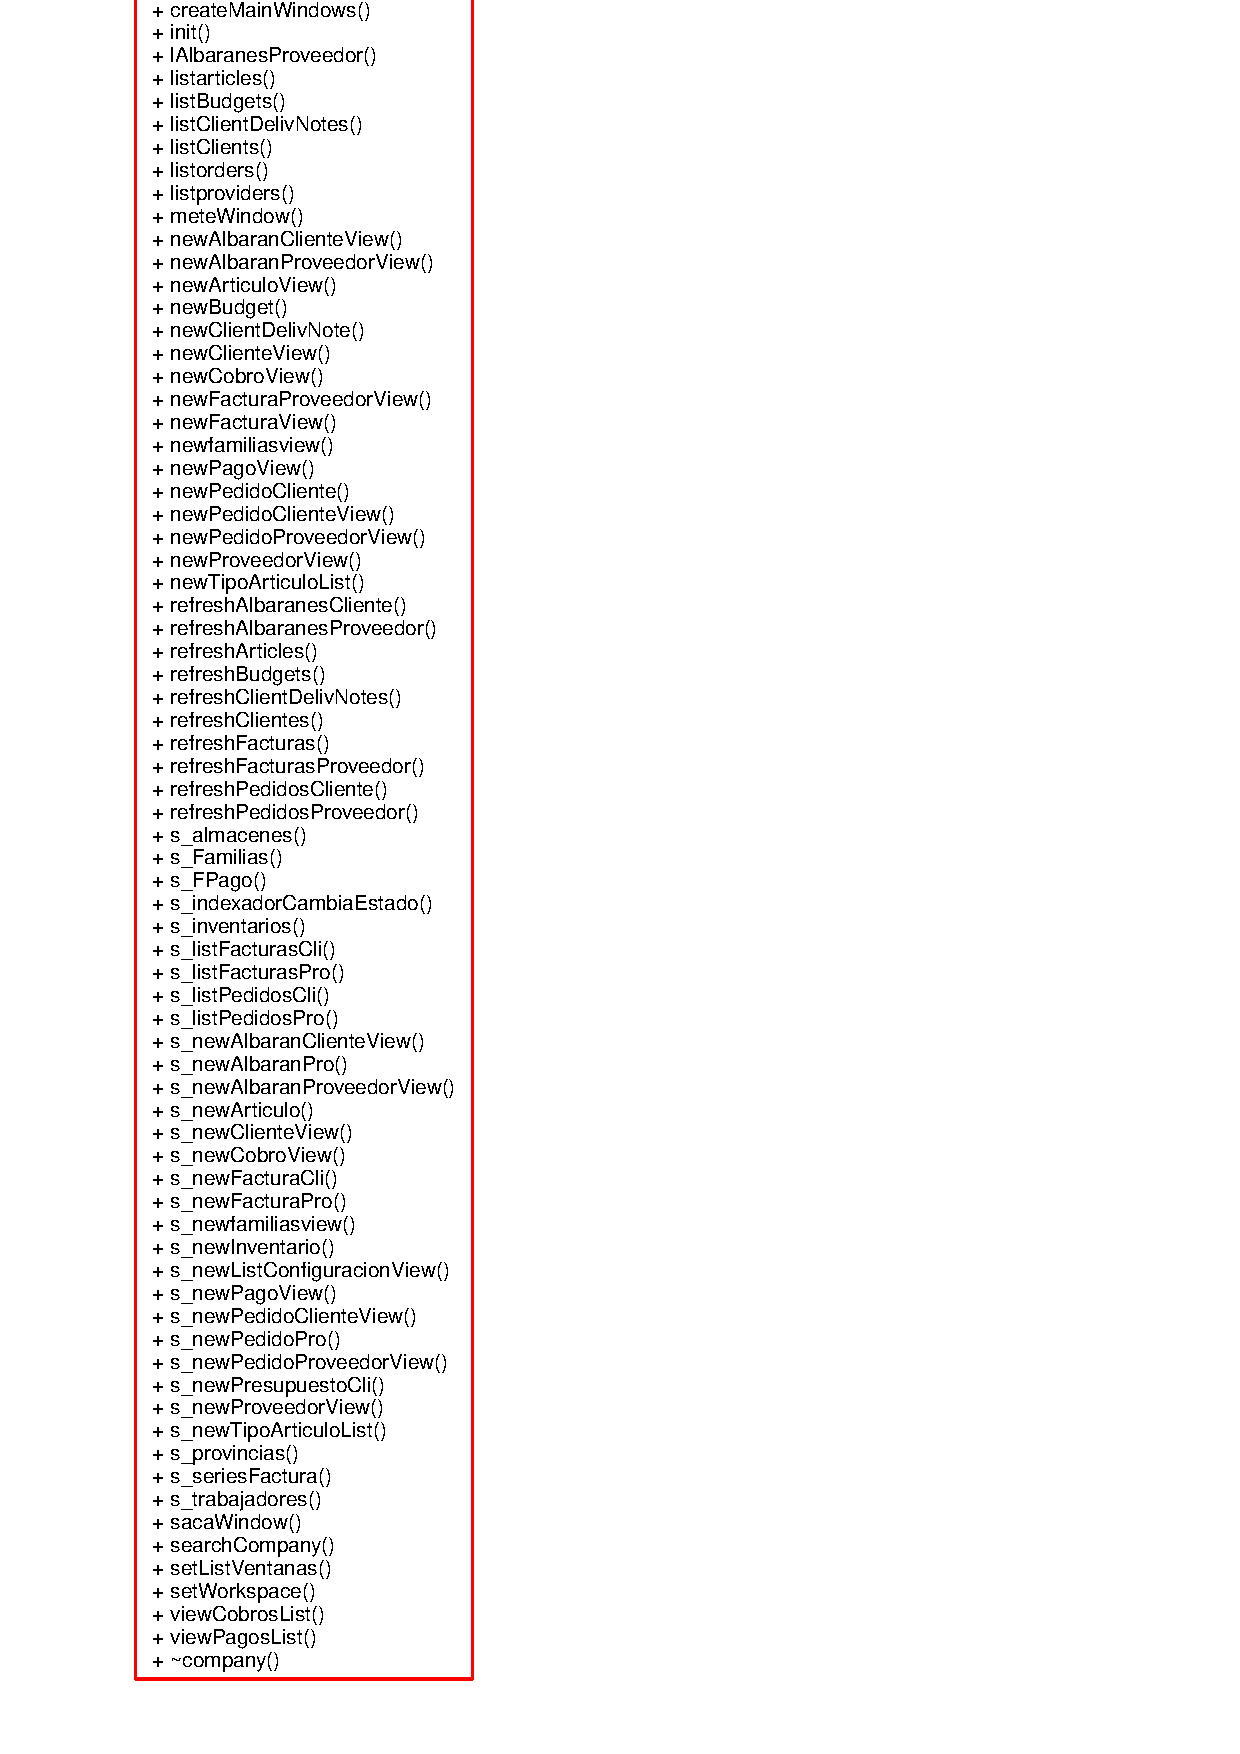
\includegraphics[width=131pt]{classCobrosList__coll__graph}
\end{center}
\end{figure}
\subsection*{Slots p\'{u}blicos}
\begin{CompactItemize}
\item 
virtual void {\bf on\_\-mui\_\-actualizar\_\-clicked} ()\label{classCobrosList_i0}

\item 
virtual void {\bf on\_\-mui\_\-borrar\_\-clicked} ()\label{classCobrosList_i1}

\item 
virtual void {\bf on\_\-mui\_\-configurar\_\-toggled} (bool checked)\label{classCobrosList_i2}

\item 
virtual void {\bf on\_\-mui\_\-crear\_\-clicked} ()\label{classCobrosList_i3}

\item 
virtual void {\bf on\_\-mui\_\-editar\_\-clicked} ()\label{classCobrosList_i4}

\item 
virtual void {\bf on\_\-mui\_\-imprimir\_\-clicked} ()\label{classCobrosList_i5}

\item 
virtual void {\bf on\_\-mui\_\-list\_\-cell\-Double\-Clicked} (int, int)\label{classCobrosList_i6}

\item 
virtual void {\bf on\_\-mui\_\-list\_\-custom\-Context\-Menu\-Requested} (const QPoint \&)\label{classCobrosList_i7}

\end{CompactItemize}
\subsection*{M\'{e}todos p\'{u}blicos}
\begin{CompactItemize}
\item 
void {\bf cargaconfig} ()\label{classCobrosList_a0}

\item 
{\bf Cobros\-List} ({\bf company} $\ast$comp=NULL, QWidget $\ast$parent=0, Qt::WFlags flag=0)\label{classCobrosList_a1}

\item 
{\bf Cobros\-List} (QWidget $\ast$parent=0, Qt::WFlags flag=0)\label{classCobrosList_a2}

\item 
QString {\bf genera\-Filtro} ()\label{classCobrosList_a3}

\item 
void {\bf guardaconfig} ()\label{classCobrosList_a4}

\begin{CompactList}\small\item\em Funciones que se encarga en guardar y cargar la configuracion del listado. \item\end{CompactList}\item 
void {\bf hide\-Botonera} ()\label{classCobrosList_a5}

\item 
void {\bf hide\-Busqueda} ()\label{classCobrosList_a6}

\item 
QString {\bf idcobro} ()\label{classCobrosList_a7}

\item 
void {\bf imprimir} ()\label{classCobrosList_a8}

\item 
void {\bf mete\-Window} (QString nom, QObject $\ast$obj)\label{classCobrosList_a9}

\item 
void {\bf modoedicion} ()\label{classCobrosList_a10}

\item 
void {\bf modoseleccion} ()\label{classCobrosList_a11}

\item 
void {\bf presentar} ()
\item 
void {\bf setcompany} ({\bf company} $\ast$comp)\label{classCobrosList_a13}

\item 
void {\bf setidcliente} (QString val)\label{classCobrosList_a14}

\item 
void {\bf show\-Botonera} ()\label{classCobrosList_a15}

\item 
void {\bf show\-Busqueda} ()\label{classCobrosList_a16}

\end{CompactItemize}


\subsection{Descripci\'{o}n detallada}
Administra los datos de la lista de cobros. 



\subsection{Documentaci\'{o}n de las funciones miembro}
\index{CobrosList@{Cobros\-List}!presentar@{presentar}}
\index{presentar@{presentar}!CobrosList@{Cobros\-List}}
\subsubsection{\setlength{\rightskip}{0pt plus 5cm}void Cobros\-List::presentar ()}\label{classCobrosList_a12}


Hacemos el calculo del total. 

La documentaci\'{o}n para esta clase fu\'{e} generada a partir de los siguientes archivos:\begin{CompactItemize}
\item 
cobroslist.h\item 
cobroslist.cpp\end{CompactItemize}
